\documentclass[]{book}

\usepackage{import}
\usepackage{preamble}
\usepackage{tikz}

\begin{document}

\noindent BECA / Huson / 11.1 IB Math SL \hspace{2in} Name:\\*
14 December 2017
\begin{center}
{\Large Take home test: Exponential functions}\\
\textit{Open notes, open book (including Wikipedia and other online materials). No online calculators or human help. Due Monday at the beginning of class.}
\end{center}

%\vspace{0.2 cm}
\subsection*{Interest rate calculations}

Use the formula for simple interest: $i=Prt$ where $P$ is the principal amount of the loan or investment in dollars; $r$ is the interest rate, usually per year but also sometimes per month; $t$ is the amount of time, in units consistent with the rate; and $i$ is the amount of interest in dollars. (round to the nearest cent)

\begin{enumerate}

\item $5\%$ interest per annum, \$10,000 principal, one year
\item $7\%$ interest per annum, \$1,500 principal, six months
\item The annual interest rate required to earn $\$200$ on \$50,000 principal in one month.

\subsection*{Functions, exponents, logs}

Simplify each expression. Leaving no negative or fractional exponents.
\item $5x^{-3}y^2 \div 2x^3 y^{2}$
\item $\sqrt[5]{x^{-10} y^{2}}$
\item $\displaystyle \left( x y^{\frac{1}{2}}\right)^4$
\item $\log_3 27$
\item $\log 5 + \log 20$
\item $\log_5 75 - \log_5 3$
\item $(2x-7)(x^2-2x-3)$

\item Let $f(x)=2x-1$ and $g(x)=-x^2+x$
\begin{enumerate}
    \item Find $f^{-1}(x)$.
    \item Find $(g \circ f)(1)$.
\end{enumerate}

\item Consider the equation $2x^2 + (k+1)x=-18$, where $k$ is a real number. Find the values of $k$ for which the equation has two equal real solutions.

\newpage
\subsection*{Exponential and quadratic functions. (calculator oriented)}

\item Let $f(x)=2x^2-5x-4$.
\begin{enumerate}
    \item Write down the coordinates of the vertex.
    \item Hence or otherwise, express the function in the form $f(x)=2(x-h)^2 +k$.
    \item Solve the equation  $f(x)=0$.
\end{enumerate}

\item Given the exponential function $\displaystyle f(x)=1.5e^{(0.03x)}$.
\begin{enumerate}
    \item Write down $f(0)$.
    \item Find $f(2)$. %solution 1.59275482...
    \item Solve for $x$ such that $f(x)=5$. %solution 40.13242681
\end{enumerate}


\item The diagram below shows the graph of a function $f$, composed of four points.

\begin{figure}[!htbp]
\begin{center}
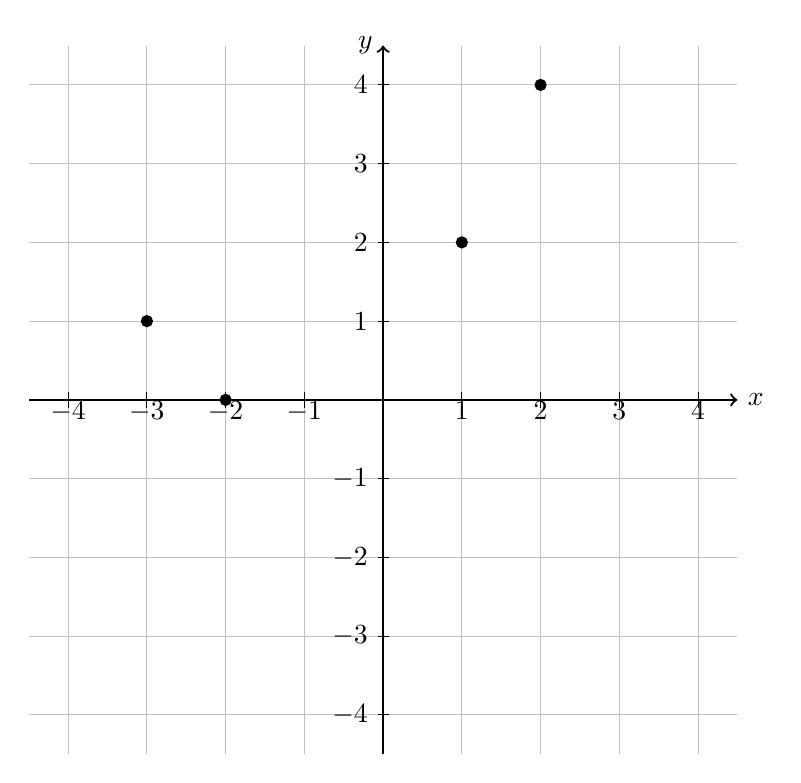
\begin{tikzpicture}

    %grid
    \draw [thin, color=lightgray,, xstep=1.0cm,ystep=1.0cm] (-4.5,-4.5) grid (4.5,4.5);
    %\draw [thin, color=lightgray,, xstep=0.2cm,ystep=0.2cm] (-4.5,-1.5) grid (5.5,16.5);
    
    \foreach \x in {-4, -3, -2, -1,1,2,3,4}
    \draw[shift={(\x,0)},color=black] (0pt,-3pt) -- (0pt,3pt) node[below]  {$\x$};
    
    \foreach \y in {-4, -3, -2, -1, 1,2,3,4}
    \draw[shift={(0,\y)},color=black] (2pt,0pt) -- (-2pt,0pt) node[left]  {$\y$};
    
    \draw [thick, ->] (-4.5,0) -- (+4.5,0) node [right] {$x$};
    \draw [thick, ->] (0,-4.5) -- (0,4.5) node [left] {$y$};
    
    \draw (-3,1) circle[radius=2pt];
    \fill (-3,1) circle[radius=2pt];
    \draw (-2,0) circle[radius=2pt];
    \fill (-2,0) circle[radius=2pt];
    \draw (1,2) circle[radius=2pt];
    \fill (1,2) circle[radius=2pt];
    \draw (2,4) circle[radius=2pt];
    \fill (2,4) circle[radius=2pt];
    
    %\draw plot[domain= -1:3] (\x, (\x+1)*(\x+1) - 4);
    
\end{tikzpicture}
\end{center}
\end{figure}

\begin{enumerate}
    \item Write down the value of $f(1)$.
    \item Write down the domain of $f$.
    \item Write down the range of $f$.
    \item Write down the value of $f^{-1}(1)$.
    \item Sketch the inverse of $f$, $f^{-1}$, on the grid above.
\end{enumerate}

\newpage
\noindent BECA / Huson / 11.1 IB Math SL \hspace{2in} Name:\\*
14 December 2017

\item Let $f$ be a quadratic function. Part of the graph of $f$ is shown below.\\*
The vertex is $P(3,2)$ and the $y$-intercept is $Q(0, -3)$.\\*

\begin{figure}[!htbp]
\begin{center}
\begin{tikzpicture}

    %grid
    %\draw [thin, color=lightgray,, xstep=1.0cm,ystep=1.0cm] (-5.5,-5.5) grid (5.5,5.5);
    %\draw [thin, color=lightgray,, xstep=0.2cm,ystep=0.2cm] (-5.5,-1.5) grid (5.5,16.5);
    
    \foreach \x in {-2, -1,1,2,3,4,5,6}
    \draw[shift={(\x,0)},color=black] (0pt,-3pt) -- (0pt,3pt) node[below]  {$\x$};
    
    \foreach \y in {-4, -3, -2, -1,1,2,3,4}
    \draw[shift={(0,\y)},color=black] (2pt,0pt) -- (-2pt,0pt) node[left]  {$\y$};
    
    \draw [thick, ->] (-2.5,0) -- (+6.5,0) node [right] {$x$};
    \draw [thick, ->] (0,-4.5) -- (0,4.5) node [left] {$y$};
    
    \draw (3,2) circle[radius=2pt] node [below] {$P$};
    \fill (3,2) circle[radius=2pt];
    \draw (0,-3) circle[radius=2pt] node [right] {$Q$};
    \fill (0,-3) circle[radius=2pt];
    
    \draw [<->] plot[domain= -0.5:6] (\x, -.555*\x*\x +3.33*\x -3);
    
\end{tikzpicture}
\end{center}
\end{figure}

\begin{enumerate}
    \item Write down the equation of the axis of symmetry.
    \item The function $f$ can be written in the form $f(x)=a(x-h)^2 +k$. \\*
    Write down the value of $h$ and of $k$.
    \item Show that $a=-\frac{5}{9}$.
    \item Find the roots of the function.
\end{enumerate}

\newpage
\item Consider the function $f(x)=x^2+2x+2$.
\begin{enumerate}
    \item Sketch the graph of $f$, for $-3 \leq x \leq 1$.
    \item This function can also be written in the form $f(x)=(x-p)^2 +1$.\\* 
    Write down the value of $p$.
    \item The graph of $g$ is obtained by reflecting the graph of $f$ in the $x$-axis, followed by a translation of $(0, 4)$.\\* Show that $g(x)=-x^2-2x+2$.
    \item The graphs of $f$ and $g$ intersect at two points.\\*
    Write down the x-coordinates of these two points.
\end{enumerate}

\begin{figure}[!htbp]
\begin{center}
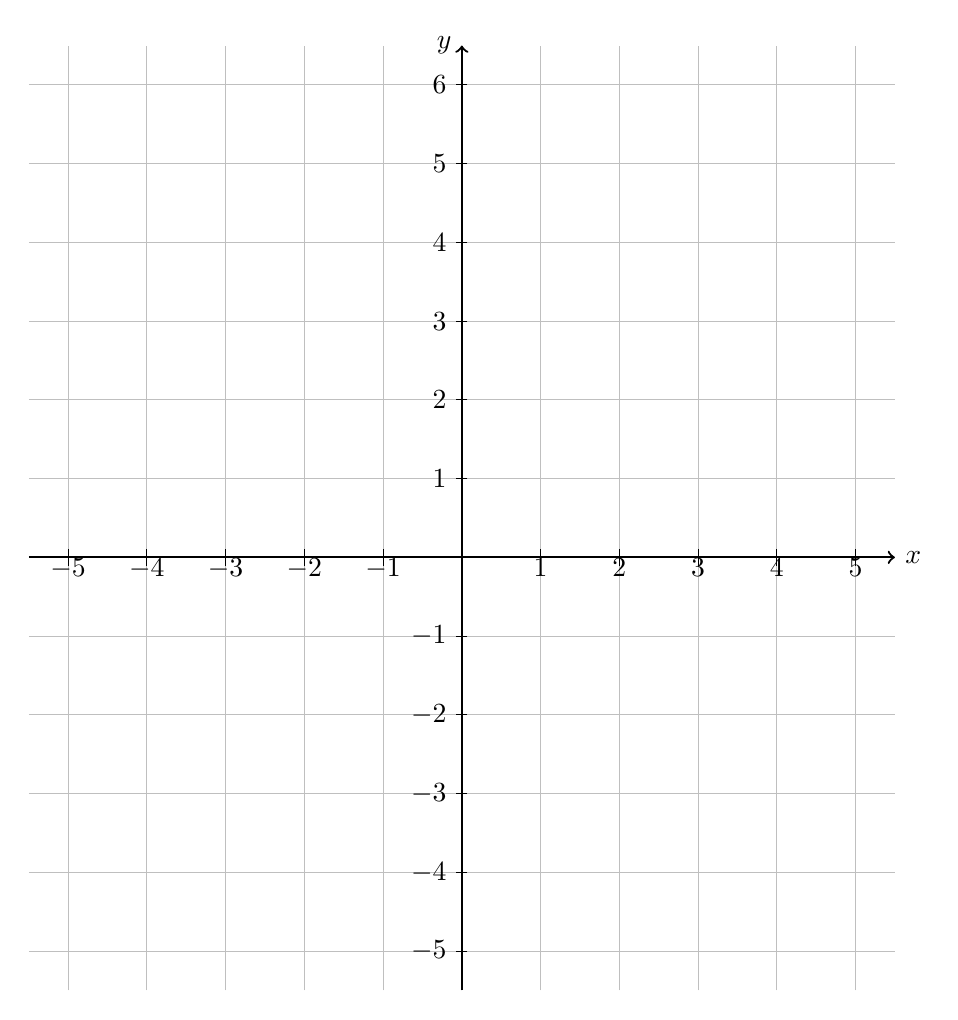
\begin{tikzpicture}

    %grid
    \draw [thin, color=lightgray,, xstep=1.0cm,ystep=1.0cm] (-5.5,-5.5) grid (5.5,6.5);
    %\draw [thin, color=lightgray,, xstep=0.2cm,ystep=0.2cm] (-4.5,-1.5) grid (5.5,16.5);
    
    \foreach \x in {-5, -4, -3, -2, -1,1,2,3,4, 5}
    \draw[shift={(\x,0)},color=black] (0pt,-3pt) -- (0pt,3pt) node[below]  {$\x$};
    
    \foreach \y in {-5, -4, -3, -2, -1, 1,2,3,4, 5, 6}
    \draw[shift={(0,\y)},color=black] (2pt,0pt) -- (-2pt,0pt) node[left]  {$\y$};
    
    \draw [thick, ->] (-5.5,0) -- (+5.5,0) node [right] {$x$};
    \draw [thick, ->] (0,-5.5) -- (0,6.5) node [left] {$y$};
    
    %\draw plot[domain= -4:2] (\x, (\x*\x +2*\x-2);
    
\end{tikzpicture}
\end{center}
\end{figure}


\subsection*{Honor pledge}
I have not received human help with this test, nor have I used calculators (including Desmos) except for an approved graphing calculator. Signed:

\end{enumerate}
\end{document}